
\documentclass{beamer}
\usepackage[utf8]{inputenc}
\usepackage[T1]{fontenc}
\usepackage{circuitikz}

\usepackage{multirow}

\title{CS241: Hardware Design}
\date{\today}
\author[Fyfe and Lynn]{Charles Fyfe and Melissa Lynn}
\institute{St Olaf College}

\usetheme{grape}

\usepackage{parskip}
\usepackage{multicol}
\usepackage{graphicx}
% make \oplus look nice
\usepackage{amssymb}

\begin{document}


\titlepage

% just sections up top
\setcounter{tocdepth}{1}

\begin{frame}{Outline}

	\begin{multicols*}{2}
		\tableofcontents
	\end{multicols*}
\end{frame}

% show subsections later
\setcounter{tocdepth}{2}


\Section{Introduction}

\Subsection{Standards-Based Grading}

\begin{frame}{Important Links}
\end{frame}
    


\Section{Data Representation}

\begin{frame}{How do computers store information?}
Computers work using electrical signals which can be on or off. If we let:
\begin{itemize}
    \item On means 1
    \item Off means 0
\end{itemize}
We can use sequences of 0s and 1s to represent information
\end{frame}

\Subsection{Positive Integers in Binary}

\begin{frame}{Numbers in Base Ten (aka Decimal)}
Let's start by talking about how we write numbers normally. 

For example, let's look at the number 109: 
\begin{align*}
109 &= 100 \;+\; 0 \;+\; 9 \\
&= 1 \times 10^2 \;+\; 0 \times 10^1 \;+\; 9 \times 10^0
\end{align*}
This way of writing numbers is called base ten.
We use ten digits (0 to 9 inclusive) and each position in the number is scaled by a power of ten.

In terms of math, there is nothing special about base ten. 
We probably use it because we have ten fingers. 
Some ancient civilizations used sompletely different systems for counting!
\end{frame}
    
\begin{frame}{Numbers in Base Two (aka Binary)}
Computers don't have fingers. They express everything as sequences of 1s and 0s. This format is called binary:

\begin{align*}
0b1101101 &= 
1 \! \times \! 2^6 +
1 \! \times \! 2^5 +
0 \! \times \! 2^4 +
1 \! \times \! 2^3 +
1 \! \times \! 2^2 +
0 \! \times \! 2^1 +
1 \! \times \! 2^0 \\
&= 64 + 32 + 0 + 8 + 4 + 0 + 1 \\
&= 109 \\
\end{align*}
Importantly: we always use the prefix ``0b'' to avoid confusion when writing numbers in binary.

1101 is one thousand one hundred and one

0b1101 is thirteen
\end{frame}

\begin{frame}{Converting from Binary to Decimal}
\end{frame}

\begin{frame}{Converting from Decimal to Binary}
\end{frame}

\begin{frame}{Addition in Binary}
Binary addition works just like decimal addition. 
Start from the right, add straight down, and carry when you run out of digits.

For example:
\[
\begin{array}{ccccccccc}
    1 & 1 & 1 & 1 & 1 &   &   &   &   \\ 
      & 0 & 0 & 1 & 1 & 1 & 0 & 0 & 0 \\ 
    + & 1 & 1 & 1 & 0 & 1 & 0 & 0 & 1 \\
    \hline
    1 & 0 & 0 & 1 & 0 & 0 & 0 & 0 & 1 \\ 
\end{array}
\]
We'll come back to subtraction later
\end{frame}

\begin{frame}{Multiplication in Binary}
Binary multiplication works just like decimal multiplication. 
Multiply the top number by the rightmost digit of the bottom number.
Then move to the next line, add a zero, and repeat for the next digit.
Finally, add up the lines. For example:
\[
\begin{array}{cccccc}
        &   &        & 1 & 1 & 0 \\ 
        &   & \times & 1 & 0 & 1 \\
    \hline
        &   &        & 1 & 1 & 0 \\ 
        &   & 0      & 0 & 0 & 0 \\
        + & 1 & 1      & 0 & 0 & 0 \\
        \hline 
        & 1 & 1      & 1 & 1 & 0 \\
\end{array}
\]
\end{frame}


\begin{frame}{Division in Binary}
To divide by 2, shift the whole number one place to the right.

To divide by 4, shift the whole number two places to the right. 

That's as deep as we go in this class. If you're curious to learn more, see the textbook.

\end{frame}

\begin{frame}{Sample Exercises}
Make sure to show your work.
\vfill 
\begin{enumerate}
    \item Convert 0b1011 from binary to decimal. 
    \vfill
    \item Convert 47 from decimal to binary.
    \vfill
    \item Add 0b1001 + 0b1011 in binary. Convert to decimal to check your work.
    \vfill
    \item Multiply 0b1101 $\times$ 0b110 in binary. Convert to decimal to verify your work.
    \vfill 
\end{enumerate}
\end{frame}

\Subsection{Negative Numbers}


\begin{frame}{First Attempt: Signed Magnitude}

We can use the first digit to hold the sign, then the rest of the digits to hold magnitue:

    \begin{itemize}
        \item 0b\Highlight{0}1011001 is positive 10110001, so 89
        \item 0b\Highlight{1}1011001 is negative 1011001, so -89 
    \end{itemize}

What are some upsides of this convention?


\end{frame}

\begin{frame}{Addition with Signed Magnitude}



\end{frame}


\begin{frame}{Subtraction with Signed Magnitude}
Subtraction is just shorthand for adding a negative number.


\end{frame}



\begin{frame}{Zero with Signed Magnitude}
\end{frame}

\begin{frame}{Another Idea: Two's Complement}
\end{frame}

\begin{frame}{Addition with Two's Complement}
\end{frame}

\begin{frame}{Zero with Two's Complement}
\end{frame}

\begin{frame}{Subtraction with Two's Complement}
\end{frame}

\begin{frame}{Sample Exercises}
Make sure to show your work.
\vfill 
\begin{enumerate}
    \item TODO
    \vfill 
\end{enumerate}
\end{frame}

\Subsection{Hexadecimal}

\Subsection{Fractions and Decimals}

\Subsection{Structured Data}

\begin{frame}{placeholder}
    strings
    audio
    images
    JSON
\end{frame}
    

% positive integers in binary
% arithmetic in binary
% negtive integers
% hex
% fractions
% structured data


\Section{Logic Representation}

\Subsection{Boolean Logic}

\begin{frame}{Bit Operations}
\end{frame}


\begin{frame}{Logic Gates}

    \begin{tikzpicture}
        % Paths, nodes and wires:
        \node[ieeestd and port] at (1.037, 10.345){};
        \node[ieeestd nand port] at (7.08, 10.375){};
        \node[ieeestd or port] at (1.143, 7.408){};
        \node[ieeestd nor port] at (7.223, 7.22){};
        \node[ieeestd xor port] at (1.106, 4.408){};
        \node[ieeestd xnor port] at (7.132, 4.345){};
        \node[ieeestd not port] at (12.877, 10.375){};
        \node[ocirc] at (-0.044, 10.625){};
        \node[ocirc] at (-0.044, 10.065){};
        \node[ocirc] at (5.999, 10.655){};
        \node[ocirc] at (5.999, 10.095){};
        \node[ocirc] at (8.161, 10.375){};
        \node[ocirc] at (2.119, 10.345){};
        \node[ocirc] at (0.061, 7.688){};
        \node[ocirc] at (0.061, 7.128){};
        \node[ocirc] at (6.141, 7.5){};
        \node[ocirc] at (6.141, 6.94){};
        \node[ocirc] at (8.304, 7.22){};
        \node[ocirc] at (2.224, 7.408){};
        \node[ocirc] at (0.025, 4.688){};
        \node[ocirc] at (0.025, 4.128){};
        \node[ocirc] at (6.051, 4.625){};
        \node[ocirc] at (6.051, 4.065){};
        \node[ocirc] at (8.213, 4.345){};
        \node[ocirc] at (2.188, 4.408){};
        \node[ocirc] at (12, 10.375){};
        \node[ocirc] at (13.75, 10.375){};
        \node[shape=rectangle, minimum width=0.215cm, minimum height=0.59cm] at (-0.448, 10.688){} node[anchor=north west, align=left, text width=-0.173cm, inner sep=6pt] at (-0.573, 11){A};
        \node[shape=rectangle, minimum width=0.215cm, minimum height=0.465cm] at (-0.448, 10.125){} node[anchor=north west, align=left, text width=-0.173cm, inner sep=6pt] at (-0.573, 10.375){B};
        \node[shape=rectangle, minimum width=0.215cm, minimum height=0.59cm] at (5.595, 10.718){} node[anchor=north west, align=left, text width=-0.173cm, inner sep=6pt] at (5.47, 11.03){A};
        \node[shape=rectangle, minimum width=0.215cm, minimum height=0.465cm] at (5.595, 10.155){} node[anchor=north west, align=left, text width=-0.173cm, inner sep=6pt] at (5.47, 10.405){B};
        \node[shape=rectangle, minimum width=0.215cm, minimum height=0.59cm] at (-0.375, 7.75){} node[anchor=north west, align=left, text width=-0.173cm, inner sep=6pt] at (-0.5, 8.062){A};
        \node[shape=rectangle, minimum width=0.215cm, minimum height=0.465cm] at (-0.375, 7.187){} node[anchor=north west, align=left, text width=-0.173cm, inner sep=6pt] at (-0.5, 7.438){B};
        \node[shape=rectangle, minimum width=0.215cm, minimum height=0.59cm] at (5.705, 7.563){} node[anchor=north west, align=left, text width=-0.173cm, inner sep=6pt] at (5.58, 7.875){A};
        \node[shape=rectangle, minimum width=0.215cm, minimum height=0.465cm] at (5.705, 7){} node[anchor=north west, align=left, text width=-0.173cm, inner sep=6pt] at (5.58, 7.25){B};
        \node[shape=rectangle, minimum width=0.215cm, minimum height=0.59cm] at (-0.442, 4.75){} node[anchor=north west, align=left, text width=-0.173cm, inner sep=6pt] at (-0.567, 5.062){A};
        \node[shape=rectangle, minimum width=0.215cm, minimum height=0.465cm] at (-0.442, 4.187){} node[anchor=north west, align=left, text width=-0.173cm, inner sep=6pt] at (-0.567, 4.437){B};
        \node[shape=rectangle, minimum width=0.215cm, minimum height=0.59cm] at (5.584, 4.688){} node[anchor=north west, align=left, text width=-0.173cm, inner sep=6pt] at (5.459, 5){A};
        \node[shape=rectangle, minimum width=0.215cm, minimum height=0.465cm] at (5.584, 4.125){} node[anchor=north west, align=left, text width=-0.173cm, inner sep=6pt] at (5.459, 4.375){B};
        \node[shape=rectangle, minimum width=0.354cm, minimum height=0.59cm] at (11.555, 10.438){} node[anchor=north west, align=left, text width=-0.034cm, inner sep=6pt] at (11.36, 10.75){A};
%        \node[shape=rectangle, minimum width=0.744cm, minimum height=0.59cm] at (14.36, 10.563){} node[anchor=north west, align=left, text width=0.356cm, inner sep=6pt] at (13.971, 10.875){$\overline{\text{A}}$};
%        \node[shape=rectangle, minimum width=0.744cm, minimum height=0.59cm] at (2.64, 4.438){} node[anchor=north west, align=left, text width=0.356cm, inner sep=6pt] at (2.25, 4.75){A\textasciicircumB};
%        \node[shape=rectangle, minimum width=0.744cm, minimum height=0.59cm] at (8.665, 4.438){} node[anchor=north west, align=left, text width=0.356cm, inner sep=6pt] at (8.276, 4.75){$\overline{\text{A^B}}$};
        \node[shape=rectangle, minimum width=0.744cm, minimum height=0.59cm] at (2.706, 7.438){} node[anchor=north west, align=left, text width=0.356cm, inner sep=6pt] at (2.317, 7.75){A|B};
%        \node[shape=rectangle, minimum width=0.744cm, minimum height=0.59cm] at (8.786, 7.313){} node[anchor=north west, align=left, text width=0.356cm, inner sep=6pt] at (8.397, 7.625){$\overline{\text{A|B}}$};
        \node[shape=rectangle, minimum width=0.744cm, minimum height=0.59cm] at (2.538, 10.375){} node[anchor=north west, align=left, text width=0.356cm, inner sep=6pt] at (2.148, 10.688){A\&B};
%        \node[shape=rectangle, minimum width=0.744cm, minimum height=0.59cm] at (8.58, 10.468){} node[anchor=north west, align=left, text width=0.356cm, inner sep=6pt] at (8.191, 10.78){$\overline{\text{A&B}}$};
        \node[shape=rectangle, minimum width=0.965cm, minimum height=0.715cm] at (0.956, 11.375){} node[anchor=north west, align=left, text width=0.577cm, inner sep=6pt] at (0.456, 11.75){and};
        \node[shape=rectangle, minimum width=0.965cm, minimum height=0.715cm] at (7.028, 11.28){} node[anchor=north west, align=left, text width=0.577cm, inner sep=6pt] at (6.528, 11.655){nand};
        \node[shape=rectangle, minimum width=0.965cm, minimum height=0.715cm] at (0.846, 8.313){} node[anchor=north west, align=left, text width=0.577cm, inner sep=6pt] at (0.346, 8.688){or};
        \node[shape=rectangle, minimum width=0.965cm, minimum height=0.715cm] at (6.955, 8.125){} node[anchor=north west, align=left, text width=0.577cm, inner sep=6pt] at (6.455, 8.5){nor};
        \node[shape=rectangle, minimum width=0.965cm, minimum height=0.715cm] at (0.775, 5.313){} node[anchor=north west, align=left, text width=0.577cm, inner sep=6pt] at (0.275, 5.688){xor};
        \node[shape=rectangle, minimum width=0.965cm, minimum height=0.715cm] at (6.83, 5.25){} node[anchor=north west, align=left, text width=0.577cm, inner sep=6pt] at (6.33, 5.625){xnor};
        \node[shape=rectangle, minimum width=0.965cm, minimum height=0.715cm] at (12.75, 11.25){} node[anchor=north west, align=left, text width=0.577cm, inner sep=6pt] at (12.25, 11.625){not};
    \end{tikzpicture}
\end{frame}



\begin{frame}{Control Circuits}

	multiplexers
\end{frame}




\Subsection{Transistors and Resistors}



\begin{frame}{Transistors}

	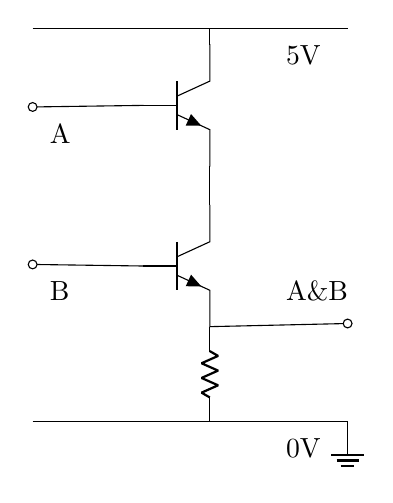
\begin{tikzpicture}
		% Paths, nodes and wires:
		\node[npn] at (5.25, 6.02){};
		\node[npn] at (5.25, 3.98){};
		\draw (5.25, 2) to[american resistor, /tikz/circuitikz/bipoles/length=0.700cm] (5.25, 3.21);
		\draw (5.25, 3.21) -- (7, 3.25);
		\draw (4.41, 3.98) -- (3, 4);
		\draw (4.41, 6.02) -- (3, 6);
		\draw (5.25, 6.79) -- (5.25, 7);
		\draw (3, 7) -- (5.25, 7) -- (7, 7);
		\draw (3, 2) -- (5.25, 2) -- (7, 2);
		\node[ground] at (7, 2){};
		\draw (5.25, 5.25) -- (5.25, 4.75);
		\node[ocirc] at (3, 6){};
		\node[ocirc] at (3, 4){};
		\node[ocirc] at (7, 3.25){};
		\node[shape=rectangle, minimum width=0.965cm, minimum height=0.215cm] at (6.5, 6.875){} node[anchor=north west, align=left, text width=0.577cm, inner sep=6pt] at (6, 7){5V};
		\node[shape=rectangle, minimum width=0.965cm, minimum height=0.215cm] at (3.5, 5.875){} node[anchor=north west, align=left, text width=0.577cm, inner sep=6pt] at (3, 6){A};
		\node[shape=rectangle, minimum width=0.965cm, minimum height=0.215cm] at (3.5, 3.875){} node[anchor=north west, align=left, text width=0.577cm, inner sep=6pt] at (3, 4){B};
		\node[shape=rectangle, minimum width=0.965cm, minimum height=0.715cm] at (6.5, 3.625){} node[anchor=north west, align=left, text width=0.577cm, inner sep=6pt] at (6, 4){A\&B};
		\node[shape=rectangle, minimum width=0.965cm, minimum height=0.465cm] at (6.5, 1.75){} node[anchor=north west, align=left, text width=0.577cm, inner sep=6pt] at (6, 2){0V};
	\end{tikzpicture}

\end{frame}



% boolean operators
% boolean expressions
% boolean circuits
% resistors & transistors


\Section{Instructions on Hardware}

\begin{frame}{Von Neumann Architecture}
	\begin{itemize}
		\item What are the fundamental parts of a computer?
		\item How do they work together to execute instructions?
	\end{itemize}
	\includegraphics[width=\columnwidth]{images/von-neumann-architecture.png}
\end{frame}

\Subsection{Hardware Components}


\begin{frame}{CPU}

	Processing unit executes program instructions. Registers for storing the very specific pieces of data you're currently using. ALU which does the actual math. For example, if you're adding two numbers. Load into r0 and r1. Send them through the ALU. Store the result in r2.

	Control unit drives execution. IR: instruction register. Holds the instruction currently being executed. PC: program counter. Holds the address of the next instruction.


	Implements the processing unit and control unit of the von Neumann architecture
	Functional units:
	The arithmetic logic unit (ALU) performs arithmetic and logic operations
	General purpose registers for storing program data
	Control circuitry and special purpose registers for instruction execution
	The clock drives the circuitry of the CPU to execute program instructions
\end{frame}


\begin{frame}{CPU}

	It's all boolean logic!

	\includegraphics[width=\columnwidth]{images/example-alu}
	\includegraphics[width=\columnwidth]{images/register-file}
	\includegraphics[width=\columnwidth]{images/full-cpu}

\end{frame}


\begin{frame}{Main Memory}
	Stores program data and instructions

	historically: tiny bits of magnetic field on a spinning disk

	modern SSD: basically a bunch of NAND gates plugged into each other

	https://en.wikipedia.org/wiki/Flash_memory#NAND_flash
\end{frame}


\begin{frame}{Busses}
	\begin{itemize}
		\item Address bus: what address in memory are we working with?
		\item Control bus: what are we doing with that address? Eg read or write
		\item Data bus: carries data between registers and memory
	\end{itemize}
\end{frame}



\begin{frame}{Input and Output}

	The input unit(s) load program data and instructions on the computer and initiate program execution.

	The output unit(s) store or receive program results.

\end{frame}





\Subsection{Clock-Driven Execution}


\begin{frame}{Clock-Driven Execution}
	\begin{itemize}
		\item Electrical signals move within the CPU, between CPU and memory, etc
		\item Different paths, different lengths, different amounts of time for signals to get where they're going
		\item CPU speed in GHz keeps everything coordinated
		\item Why not just make the clock run faster? Speed of light
	\end{itemize}
\end{frame}


\Subsection{Executing an Instruction}





\Subsection{Locality and Cache}



\begin{frame}{The Memory Hierarchy}
	\includegraphics[width=\columnwidth]{images/memory-hierarchy-books.png}
\end{frame}

\begin{frame}{The Memory Hierarchy}
	\includegraphics[width=\columnwidth]{images/memory-hierarchy.png}
\end{frame}

\begin{frame}{What is a cache?}
	\begin{itemize}
		\item Cache holds data that you are likely to want soon. Recent and/or adjacent.
		\item spatial locality
		\item temporal locality
		\item A CPU generally has a few layers of cache
	\end{itemize}
\end{frame}

\begin{frame}{Important terms}
	\begin{itemize}
		\item Primary storage
		\item Secondary storage
		\item Latency
		\item Capacity
		\item Transfer rate (aka throughput)
	\end{itemize}
\end{frame}



\Subsection{Pipelining and Hazards}









\Subsection{Executing Instructions}

\begin{frame}{FDEW}

	\begin{itemize}
		\item Fetch. Read the instruction from memory into IR (in the control unit of the CPU)
		\item Decode. Set up the processing unit to perform the instruction. Send the instruction to the ALU, open gates to send appropriate registers to ALU inputs
		\item Execute. Send the inputs and the instruction into the ALU, which computes the result
		\item Write. Store the results from the ALU
	\end{itemize}

\end{frame}

\begin{frame}{Fetch}
	\includegraphics[width=\columnwidth]{images/fdew-fetch}

	The control unit fetches the next instruction from memory.
	The special register pc (program counter) in the control unit contains the address of the next instruction.
	That address is sent on the address bus, from the control unit to memory.
	The READ command is sent on the control bus, from the control unit to memory.
	The memory unit reads the instruction at the given address, and sends them on the data bus to the control unit. The instruction is stored in the special register ir (instruction register).
	The control unit increments the value of pc to the address of the next instruction.


\end{frame}

\begin{frame}{Decode}
	\includegraphics[width=\columnwidth]{images/fdew-decode}

	The control unit decodes the instruction.
	After the fetch phase, the instruction is in the special register ir (instruction register) of the control unit.
	The control unit decodes the operation to perform and the location of the operands from the instruction.
	The control unit tells the processing unit what operation to perform.
	The control unit fetches data operand values from their locations (CPU registers, memory, or instruction bits), sends as inputs to the processing unit.
	(Often) no information sent over buses (between CPU and Memory).

\end{frame}

\begin{frame}{Execute}
	\includegraphics[width=\columnwidth]{images/fdew-execute}

	The processing unit executes the instruction.
	In the processing unit, the ALU (arithmetic logic unit) performs the instruction operation on the instruction data operands (now stored in registers).
	No information sent over buses (between CPU and Memory).

	NOTE: this is the only part of the cycle that actually does any "real" work! The rest is overhead and bookkeeping
\end{frame}

\begin{frame}{Write}
	\includegraphics[width=\columnwidth]{images/fdew-write}

	The control unit stores the result of the executed instruction to memory.
	The resulting value is sent on the data bus, from the control unit to memory.
	The address of the storage location is sent on the address bus, from the control unit to memory.
	The WRITE command is sent on the control bus, from the control unit to memory.
	When the memory unit receives this information, it writes the value to memory at the specified address.

	NOTE: write to memory vs writeback to registers. these both happen as necessary after execute. don't worry too much about it. we'll talk a bit more in memory hierarchy
\end{frame}


\begin{frame}{Clock-Driven Execution}
	\begin{itemize}
		\item Each step takes one CPU cycle
		\item CPU speed is measured in GHz
		\item 1 MHz = 1 million cycles per second
		\item 1 GHz = 1 billion cycles per second
	\end{itemize}

	In the CPU, the clock drives the execution of instructions.
	Used to determine when circuits from each stage become available.
	Used to determine when outputs are ready to be inputs for next stage.
	Time is discrete, not continuous. There is time 0, 1, 2, … but no time 1.5.
	The processor's clock cycle time is the time between each clock tick. Units: seconds, nanoseconds, etc.
	The processor's clock speed (or clock rate) is 1/(clock cycle time); the number of clock ticks per second. Units: megahertz, gigahertz, etc.
	1 MHz = one million clock ticks per second
	1 GHz = one billion clock ticks per second

\end{frame}


\begin{frame}{Why not just make the clock run faster?}

	\begin{itemize}
		\item Electricity moves at approximately the speed of light
		\item Speed of light is about one foot per nanosecond
		\item If the computer runs at 1 GHz, that's one cycle every nanosecond
		\item Wires in the CPU are twisted and packed very tightly. How long do you suppose they would be if straightened?
	\end{itemize}
\end{frame}


\begin{frame}{Von Neumann Bottleneck}
	Suppose you have an array of a billion integers in memory. You want to add 1 to each of them. How do you do it?
\end{frame}


\begin{frame}{foo bar}
	\includegraphics[width=\columnwidth]{images/instruction-breakdown}
	\begin{itemize}
		\item fizz
		\item buzz
	\end{itemize}
\end{frame}

\begin{frame}{foo bar}
	\includegraphics[width=\columnwidth]{images/fdew-add-fetch}
	\begin{itemize}
		\item Memory address of the next instruction is stored in the special register pc (program counter). 
		\item The CPU fetches the that instruction from memory into the special purpose register ir (instruction register). 
		\item The address in pc is incremented, to hold the address of the next instruction.
	\end{itemize}
\end{frame}

\begin{frame}{Walkthrough: Decode}
	\includegraphics[width=\columnwidth]{images/fdew-add-decode}
	\begin{itemize}
		\item The CPU breaks down the instruction bits from IR into its component parts
		\item The opcode is sent to the ALU
		\item Sources and destination are sent to the register file
	\end{itemize}
\end{frame}

\begin{frame}{Walkthrough: Execute}
	\includegraphics[width=\columnwidth]{images/fdew-add-execute}
	\begin{itemize}
		\item ALU performs the operation on the operands
		\item ALU outputs result and condition code values associated with the result value.
	\end{itemize}
\end{frame}

\begin{frame}{Walkthrough: Write(back)}
	\includegraphics[width=\columnwidth]{images/fdew-add-write}
	\begin{itemize}
		\item Result from ALU is stored in destination register
	\end{itemize}
\end{frame}




\begin{frame}{Eager Execution Gone Wrong}
    \includegraphics[width=\columnwidth]{images/xkcd-meltdown-cropped.png}
\end{frame}

% parts of a computer
% memory hierarchy
% executing instructions
% the von neumann bottleneck
% clock-driven execution
% instruction walkthrough
% pipelining
% data hazards
% control hazards

\input{sections/assembly-globals.tex}
% why study assembly?
% global variables
% mov
% printf
% ldr
% scanf
% add, mul

\input{sections/os-concepts.tex}
% booting
% forking
% threads, cores, processes
% async

\Section{Assembly Functions}


\begin{frame}{Push and Pop}

	When a program starts running, the OS loads the instructions into memory.

	It also allocates memory for the program to use during execution

	There is a special register called the stack pointer which provides the location of that memory

\end{frame}





\begin{frame}{Working Memory}
	\begin{columns}
		\begin{column}{0.5\textwidth}

			we do not know what piece of memory the OS will provide

			arbitrarily say it starts at 0x5000

			stack pointer points to the "bottom" of our available memory. we work our way "up" by subtracting from the stack pointer

		\end{column}
		\begin{column}{0.5\textwidth}
			\begin{alltt}
				\begin{tabular}{ r | l }
					0x4ff8 & \vdots           \\
					0x4ffc & available        \\
					0x5000 & available        \\
					0x5004 & in use by parent \\
					0x5008 & in use by parent \\
					0x500c & \vdots           \\
				\end{tabular}
			\end{alltt}
		\end{column}
	\end{columns}

\end{frame}


\begin{frame}{Branch and Link}

	New command: BL

	Branch and Link

	Branch = modify PC. Recall: PC tells us what to do next. Usually we just do the next line. In this case, we will jump to some other part of the program. This is how we call a function.

	Link = set LR to the PC of the next line. Once we're done with the function, this is how we return to the parent context.

\end{frame}


\begin{frame}{Stack Frame Walkthrough}
	\small
	\begin{columns}
		\begin{column}{0.5\textwidth}
			\begin{alltt}
				\begin{tabular}{r | l}
					       & {\quad}.section .rodata \\
					       &                         \\
					       & {\quad}.text            \\
					       & func:                   \\
					0x3fd4 & {\quad}push \{fp, lr\}  \\
					0x3fd8 & {\quad}add fp, sp, \#4  \\
					0x3fdc & {\quad}sub sp, sp, \#8  \\
					0x3fe0 & {\quad}...              \\
					0x3fe4 & {\quad}sub sp, fp, \#4  \\
					0x3fe8 & {\quad}pop \{fp, pc\}   \\
					       &                         \\
					       & {\quad}.global main     \\
					       & main:                   \\
					0x3fec & {\quad}push \{fp, lr\}  \\
					0x3ff0 & {\quad}add fp, sp, \#4  \\
					0x3ff4 & {\quad}sub sp, sp, \#12 \\
					0x3ff8 & {\quad}bl func          \\
					0x3ffc & {\quad}sub sp, fp, \#4  \\
					0x4000 & {\quad}pop \{fp, pc\}   \\
				\end{tabular}
			\end{alltt}
		\end{column}
		\begin{column}{0.5\textwidth}
			\begin{alltt}
				\begin{tabular}{ r | l}
					\vdots & \vdots    \\
					0x4ffc & available \\
					0x5000 & available \\
					0x5004 & in use    \\
					\vdots & \vdots    \\
				\end{tabular}
			\end{alltt}

			\vspace{1cm}

			\begin{alltt}
				\begin{tabular}{ r | l}
					sp & 0x5004    \\
					fp & parent fp \\
					pc & 0x3fec    \\
					lr & parent lr \\
				\end{tabular}
			\end{alltt}
		\end{column}
	\end{columns}

\end{frame}



% memory diagrams
% the stack
% calling a function
% stack frames
% bl
% push, pop
% nested function calls

\Section{Assembly Conditionals and Loops}

% b, beq, bne, ...
% if/else
% while loops
% for loops

\input{sections/networking.tex}


% 
\Section{Appendix}


\Subsection{Raspberry Pi Setup}


\begin{frame}{Pi Setup: Kit Contents}
	\begin{columns}
		\begin{column}{0.5\textwidth}
			\begin{enumerate}
				\item Pi case
				\item Raspberry Pi (in box)
				\item Heat sinks
				\item Power cord
				\item Ethernet to USB adapter
				\item Ethernet cord
				\item USB 2 to USB 3 adapter
				\item SD Card
				\item Accessory case
			\end{enumerate}
		\end{column}
		\begin{column}{0.5\textwidth}
			\includegraphics[width=\columnwidth]{images/pi-kit-contents}
		\end{column}
	\end{columns}
\end{frame}


\begin{frame}{Pi Setup: Apply Heat Sinks}
	\begin{columns}
		\begin{column}{0.5\textwidth}
			\includegraphics[width=\columnwidth]{images/pi-heat-sinks-1}
		\end{column}
		\begin{column}{0.5\textwidth}
			\includegraphics[width=\columnwidth]{images/pi-heat-sinks-2}
		\end{column}
	\end{columns}
\end{frame}

\begin{frame}{Pi Setup: Apply Nonslip Nubs}
	\includegraphics[width=\columnwidth]{images/pi-case-nubs}
\end{frame}

\begin{frame}{Pi Setup: Install in Case}
	\includegraphics[width=\columnwidth]{images/pi-in-case}
\end{frame}

\begin{frame}{Pi Setup: SD Card}
	\begin{columns}
		\begin{column}{0.5\textwidth}
			\includegraphics[width=\columnwidth]{images/pi-sd-card-1}
		\end{column}
		\begin{column}{0.5\textwidth}
			\includegraphics[width=\columnwidth]{images/pi-sd-card-2}
		\end{column}
	\end{columns}
\end{frame}

\begin{frame}{Pi Setup: Connect to Laptop}
	\includegraphics[width=\columnwidth]{images/pi-to-laptop}
\end{frame}

\begin{frame}{Pi Setup: Connect to Power}
\end{frame}

\begin{frame}{Laptop Setup: Enable WiFi}
	\includegraphics[width=\columnwidth]{images/pi-network-settings}
\end{frame}

\begin{frame}{Laptop Setup: Install VSCode}
	\includegraphics[width=\columnwidth]{images/vscode-remote-ssh}
\end{frame}

\begin{frame}{Laptop Setup: Add Remote Connection}
	\includegraphics[width=\columnwidth]{images/vscode-add-remote}
\end{frame}

\begin{frame}{Laptop Setup: SSH Login}
	\begin{itemize}
		\item Default username/password is raspberri/pi
		\item Make sure to update username and password
	\end{itemize}
\end{frame}


\Subsection{CSGit Setup}

% vscode setup
% pi setup
% csgit setup


\end{document}